\chapter{Why One Graph Is Never Enough}
\label{ch:why-one-graph-is-never-enough}

I have never worked with a team that set out to build a distributed graph.
Every federated graph I have seen started as one GraphQL service that worked,
and it usually kept working for longer than anyone later admitted. The service
got busy, the company hired, and at some point shipping a field to production
started to involve three teams and a scheduling conversation. Federation is
what people reach for at that point.

So this chapter is not a sales pitch. It is the argument the rest of the book
depends on, and it has three moving parts: what a single schema actually gives
you, what starts to fail once enough teams share it, and what federation
charges you for the fix. I will introduce Mosaic, the storefront we build and
then pull apart over the following chapters, and I will end by trying to talk
you out of all of it. Chapter~\ref{ch:do-you-actually-need-federation} makes
that case properly, with the alternatives worked through. Here I only want you
to be suspicious.

\section{The promise of one graph}
\label{sec:ch01-promise}

The pitch that got GraphQL into so many companies had nothing to do with
distribution. It was that a client could ask for exactly the data a screen
needed, once, and get back a response shaped like the screen.

\begin{minted}{graphql}
# Sketch: one request for a product page. This is the promise that made
# GraphQL spread, and it is worth keeping in view for the whole chapter.
query ProductPage($sku: String!) {
  product(sku: $sku) {
    title
    description
    price { amount currency }
    availableQuantity
    reviews(first: 3) { nodes { rating body } }
  }
}
\end{minted}

Anyone who has assembled that page from four REST endpoints, each returning a
slightly different notion of a product, each with its own pagination style and
its own opinion about whether \code{null} means missing or zero, understands the
appeal immediately. The mobile team stops asking the backend team for a new
endpoint every sprint. The backend team stops maintaining nine variants of
\code{/product} that differ only in which fields they include. Nobody has to
negotiate a payload.

That is the part everyone remembers. The part that matters more for this book is
the second promise, which is organisational rather than technical. If there is
one schema, there is one place where the company's domain is written down.
\code{Product} means one thing. \code{Money} has one shape. When somebody asks
what data the company has about a customer, the answer is a document that is
guaranteed to be current, because it is the thing serving traffic. Apollo made
this the first of its principles for running GraphQL at scale, arguing that a
company should have \enquote{one unified graph, instead of multiple graphs
created by each team}~\autocite{schmidt2019principled}. The instinct is right,
whatever you make of the source: a single graph is worth more than several
disconnected ones, because the value is in the
joins.\index{one graph principle}

\index{schema!as shared vocabulary}%
For a while, this works beautifully, and it is worth being precise about why,
because the reason is not technical merit. It is that coordination is free when
the graph is small. One team owns the schema. The people who would need to
agree about \code{Product} sit near each other, or at least attend the same
standup. A field gets added in the morning and ships in the afternoon. If
somebody proposes a name that will age badly, the person who will suffer for it
is in the room and says so.

Under those conditions a single GraphQL service is close to the best available
architecture, and I want to be clear that I mean that. Nothing in the following
twenty-seven chapters is an argument that you should have started differently.
The correct first move is one service, one schema, one deployable. The problems
this book solves are the problems of success: more teams, more domains, more
people with a legitimate claim on the same types.

\index{coordination cost}%
What changes is not the code. A schema with four hundred fields is not
meaningfully harder to compile than one with forty. What changes is the number
of people who have to agree before a field can move, and that number grows
faster than the schema does. Ten engineers on one graph is a conversation.
Eighty engineers on one graph is a queue.

Figure~\ref{fig:ch01-one-schema-many-teams} is the shape of that queue. It is
worth looking at for a moment, because it is an unremarkable diagram of an
unremarkable architecture, and everything that goes wrong in the next section
is already visible in it.

\begin{figure}[htbp]
  \centering
  % Many teams, one schema file, one deployable. Referenced from chapter 01.
% Bare tikzpicture: the figure environment, caption and label live at the
% call site. Uses only arrows.meta and positioning (loaded in packages.tex).
\begin{tikzpicture}[
    font=\small,
    team/.style={draw, rounded corners=2pt, minimum width=21mm,
                 minimum height=7mm, align=center},
    core/.style={draw, thick, minimum width=76mm, minimum height=11mm,
                 align=center},
    consumer/.style={draw, dotted, minimum width=21mm, minimum height=7mm,
                     align=center},
    flow/.style={-{Stealth[length=2mm]}, thick},
    note/.style={font=\scriptsize\itshape, align=left}
  ]

  \node[team] (t1) at (-3.45,2.1) {Catalog};
  \node[team] (t2) at (-1.15,2.1) {Orders};
  \node[team] (t3) at ( 1.15,2.1) {Pricing};
  \node[team] (t4) at ( 3.45,2.1) {Accounts};

  \node[core] (schema) at (0,0) {one schema, one deployable};

  \foreach \t in {t1,t2,t3,t4}{%
    \draw[flow] (\t) -- (schema);
  }

  \node[consumer] (web) at (-2.3,-2.1) {web};
  \node[consumer] (ios) at ( 0,-2.1) {iOS};
  \node[consumer] (part) at ( 2.3,-2.1) {partners};

  \foreach \c in {web,ios,part}{%
    \draw[flow] (schema) -- (\c);
  }

  \node[note, anchor=west] at (4.3,1.05)
    {every change is a PR\\against the same file};
  \node[note, anchor=west] at (4.3,-1.05)
    {every change ships\\on the same deploy};

\end{tikzpicture}

  \caption{One schema and one deployable, shared by every team that has
  anything to say about the domain. The arrows into the box are the ones that
  cause trouble: every change is a pull request against the same file, and
  every change ships when the whole service ships.}
  \label{fig:ch01-one-schema-many-teams}
\end{figure}

\section{Where the single schema cracks}
\label{sec:ch01-cracks}

What follows is not a list of things that might go wrong. Each item has a
company's name and a date on it, because \enquote{the monolith was fine} is an
argument I have had several times, and it is easier to have with sources.

\index{schema!review contention}%
Start with the review queue, because it is the first thing anybody notices.
Booking.com described their pre-federation GraphQL service plainly: as it grew,
one team was left with \enquote{dozens of merge requests a day to review for
schema changes and service mappings}, while also managing frequent deployments
of that service and helping resolve merge conflicts between
teams~\autocite{ernst2022booking}. The detail I find most useful is what this did
to ownership. In their words, it \enquote{made it difficult for service owners
to have strong ownership of their data and schema as they were heavily tied to
the single service}. The teams that understood a domain were not the teams that
could change how it was exposed. Ownership had become a label rather than a
capability.

\index{API monolith}%
The second failure mode is the one I would put on a poster, and Netflix has the
clearest telling of it because they walked into it having already done the hard
work of avoiding it. They had broken their system into microservices, and then,
as Jennifer Shin put it in a 2020 talk, found that those services were
\enquote{all aggregated into a single API monolith}. Her colleague Stephen
Spalding described how it happened: the gateway that composed all those services
kept acquiring responsibilities, fallback logic to handle failure gracefully,
then caches, then in-memory datastores, then business logic, until \enquote{the
API gateway had become the new monolith}~\autocite{shin2020netflixtalk}.

That is worth sitting with, because nothing in it is about GraphQL. Any
aggregation layer with one owner and many contributors drifts toward becoming
the system's centre of gravity. GraphQL just makes the drift legible, since the
accumulated coupling has a name and a file you can open.

\index{schema!quality decay}%
Third, schema quality decays when the people who own the schema are not the
people who own the domain. Netflix's account of their Studio API bottlenecks
names three causes: the API team was \enquote{disconnected from the domain
expertise and the product needs, which negatively impacted the schema's
health}; wiring a new back-end element into the graph was manual work that
\enquote{ran counter to the rapid evolution promised by a microservice
architecture}; and one small team could not keep up with the operational and
support burden of a growing graph~\autocite{shikhare2020netflix1}. The
consequence they report is the kind of thing that never appears in an
architecture diagram: inconsistent data across Studio applications was the top
support issue in their studio engineering organisation in 2018. A modelling
problem had turned into a support queue, which is usually how modelling problems
announce themselves.

\index{deploy coupling}%
Fourth, deploy coupling, which in practice means two teams have to ship before
one field exists. Tejas Shikhare put the fix in terms of the problem: with
federation, \enquote{you don't have to implement the feature in the backend
service, in the GraphQL service before the client can use it}, so the team that
owns the data can ship it and it is simply
there~\autocite{shikhare2023podcast}. Volvo Car Mobility described the same
tax from the other side: every schema change meant working inside the monolith
\emph{and} defining service-to-service APIs \emph{and} changing one or more
microservices, and on top of that their uptime depended on that single
service~\autocite{radjavi2023volvo}.

\index{breaking changes}%
Fifth, and this one is quieter, you eventually cannot change anything because
you do not know who is reading it. Matt Oliver of Major League Baseball
described having \enquote{low visibility into who is making calls on our
platform}, with clients owned by different teams, which made model changes and
breaking changes hard, because notifying and coordinating those clients was
itself the difficult part~\autocite{oliver2022mlb}. I want to flag an honest
caveat here: federation does not fix this. What fixes it is a schema registry
and operation-level tracking, which federated tooling tends to bring along
because composition needs a registry anyway. You can have that without
federating, and chapter~\ref{ch:do-you-actually-need-federation} says so.

\index{velocity ceiling}%
The cumulative version is a ceiling that hiring does not raise. Wayfair's Leah
Hurwich Adler, describing their monolith to Apollo, said it was \enquote{so
unwieldy that we hit a ceiling in our velocity, and hiring more engineers didn't
help us push code to production faster}~\autocite{adler2024wayfair}. That
sentence is the shape of the whole problem. If throughput were limited by
engineering capacity, more engineers would help. It was limited by a shared
resource, and adding contenders for a shared resource makes the contention
worse.

The most candid summary I know comes from PayPal in 2019, early enough that the
author was not describing a solved problem. Mark Stuart wrote that users
reasonably want \enquote{a single, cohesive graph that they can traverse through
without thinking about many services}, and then immediately conceded: \enquote{In
reality, assembling a single graph is difficult.} He calls it \enquote{the most
difficult problem that we have with GraphQL}, and locates the difficulty
correctly: \enquote{scaling in the Enterprise isn't about horizontal scaling or
paying a lot of money for servers or cloud compute. Scaling people, tooling and
processes are most challenging}~\autocite{stuart2019paypal}.

Now read back over that list and notice what is missing from it. Not one of
these is a performance problem, and not one is a limitation of GraphQL as a
language. They are all questions about who is allowed to change what, and how
long everyone else waits while they do. That is a specific kind of problem with
a specific and well known cause, which is the next section.

\section{The org chart in your schema}
\label{sec:ch01-org-chart}

\index{Conway's law}%
In 1968 Melvin Conway published an observation that has outlived almost
everything else written about software that decade: organisations which design
systems are constrained to produce designs which are copies of the
communication structures of those organisations~\autocite{conway1968committees}.
He was writing about committees and contract negotiations, not APIs, and the
paper is worth reading partly because it is so unlike the slogan it turned
into.

The same paper contains the arithmetic that explains the queue at the end of
section~\ref{sec:ch01-promise}, and I had somehow never noticed it until I went
back to the original. Conway points out that the number of possible
communication paths in an organisation is roughly half the square of the number
of people in it, and draws the conclusion himself: \enquote{Even in a moderately
small organization it becomes necessary to restrict communication in order that
people can get some `work' done.} Restricting communication is what a review
process is. It is not bureaucracy arriving to spoil things; it is the only way a
group above a certain size can ship anything at all.

A GraphQL schema is an unusually literal demonstration. The schema is the
interface, and it is a single document. If six teams contribute to one
document, then those six teams need a communication structure capable of
reaching agreement about that document, and they will build one whether anybody
plans it or not.

You can usually see what they built. Look for a schema working group with a
standing meeting, a naming conventions page that is longer than it should be, a
rule that schema changes need approval from two reviewers outside the
contributing team, an RFC template for adding a type. None of this is
dysfunction. It is a reasonable organisation noticing that a shared artifact
needs shared governance and supplying some. I have helped build these processes
and would build them again.

Both of those descriptions are drawn from life. Netflix ran a schema working
group that met weekly, with a schema architect whose job was to understand the
entire surface area of the graph~\autocite{shin2020netflixtalk}, and they were
straightforward about the trade: \enquote{while reviews add overhead to the
product development process}, they judged that protecting the quality of the
model would cost less later~\autocite{shikhare2020netflix2}. PayPal, once
GraphQL had spread widely enough inside the company, established a standards
body, and reported the bill just as plainly: adoption of the one-graph approach
\enquote{has been slow}, because teams \enquote{have to change a lot of
behavior}, which adds \enquote{process and time to
deliver}~\autocite{kapoor2021paypal}.

They also work. That is the part usually left out of the argument for
federation, so let me put it in early: process solutions to schema coupling are
cheap, effective, and correct for far longer than vendors suggest. If your
complaint is inconsistent field naming, you do not have a distribution problem.
You have a style guide problem, and adopting federation to solve it means paying
for a router and a schema registry to avoid writing a document.
Chapter~\ref{ch:do-you-actually-need-federation} returns to this with the
alternatives worked out properly, because the honest
answer for a lot of teams is that better governance of one graph beats a
federated graph they are not ready to operate.

\index{schema!governance}%
What governance cannot fix is the second arrow in
figure~\ref{fig:ch01-one-schema-many-teams}. You can make review faster. You
can make ownership unambiguous with a \code{CODEOWNERS} file. You cannot make
two teams ship the same binary at different times. Deploy coupling is not a
communication problem, so no amount of communication resolves it, and it is the
one failure mode that gets monotonically worse as the organisation grows.

There is a related trap worth naming, because it is where the coupling starts to
distort the schema itself. When adding a field to an existing type is expensive,
people stop adding fields to existing types. They add
\code{productPricingDetails} alongside \code{product} because a new root field
touches nobody else's code and needs one reviewer. The schema slowly grows a
layer of near-duplicate types whose only reason for existing is that they were
cheaper to merge than the correct change would have been. A year later the graph
is genuinely confusing to clients, and the cause was not incompetence. It was
that the org chart made the right change expensive and the wrong change free.

\index{team autonomy}%
Turned around, this is the actual argument for federation, and it is worth
stating in Conway's terms rather than in terms of performance or scale, neither
of which federation reliably improves. If you want teams that can decide and
ship independently, you need interfaces they can change independently. A single
schema gives you one interface with many owners. Federation gives you many
interfaces, each with one owner, plus machinery that presents them to clients as
though they were still one graph. That machinery is the cost. The independence
is what you are buying.

Whether the trade is worth it depends on how many teams you have and how often
they collide, which is a question about your organisation that no benchmark will
answer. Section~\ref{sec:ch01-do-you-need-this} gives you a way to interrogate
it, and the exercise at the end of the chapter turns it on your own graph.

\section{From stitching to federation}
\label{sec:ch01-stitching-to-federation}

When Facebook open-sourced GraphQL in 2015, the specification described a
language for asking one server for data~\autocite{byron2015graphql}. It had
nothing to say about how several teams should build that server together,
because at the time that was not the problem anybody had. The problem arrived
about two years later, and the industry has been working on it ever since. The
history is worth a few pages, because both of the answers people tried are
still in use, and the difference between them is the difference between a
gateway you maintain and a gateway you configure.

\subsection*{Stitching}
\index{schema stitching}

Apollo published the first answer in September 2017. Schema stitching was, in
Sashko Stubailo's description, \enquote{the idea that you can take two or more
GraphQL schemas, and merge them into one endpoint that can pull data from all
of them}~\autocite{stubailo2017stitching}. It shipped as a stable feature that
October in \code{graphql-tools} 2.0, with three moving
parts~\autocite{novikov2017tools2}: introspect a remote API and turn it into a
local schema object, merge several such schemas into one, and write resolvers
by hand to link types that live in different backends.

That last part is the one to hold on to. If \code{Order} lived in one service
and \code{User} in another, the code that taught the graph how to get from an
order to its customer was written in the gateway, by whoever owned the gateway.

Stitching had a real virtue, and it is the reason its descendants are still
around. It asked nothing of the services being stitched. Any spec-compliant
GraphQL API could be absorbed without knowing it had been absorbed, which is
exactly what you want when you are aggregating things you do not control, such
as a vendor's API or a service belonging to a team that has no interest in your
architecture.

What it did not fix was the queue from section~\ref{sec:ch01-org-chart}. It
moved it. Instead of six teams editing one schema file, six teams now needed
changes in one gateway repository, and the gateway's resolvers encoded
assumptions about types those teams owned. Apollo's 2018 release added a
transform layer, which made the glue more capable and also gave it more surface
area to be wrong about~\autocite{stubailo2018nextgen}.

The sharpest contemporary statement of the problem came from Marc-Andr\'e
Giroux in October 2018, six months before federation existed, which is part of
why I trust it more than the migration stories that came later. He observed
that a large stitched schema ends up with \enquote{a lot of `glue' code at the
gateway itself, defining all the important relations there}, that
responsibility drifts until the gateway becomes \enquote{responsible of
everything}, and then asked the question that has never really been answered on
stitching's own terms: \enquote{what is the point of having decentralized
schemas when in reality, we need a centralized point to merge and extend the
schemas?} He also noticed the cost that shows up in a developer's week rather
than an architecture review, which is that linking a new field to another
service now takes two steps instead of one, once at the service and again at
the gateway~\autocite{giroux2018stitching}.

Expedia's account of migrating off stitching names the operational version of
the same thing: their gateway code kept getting more complex, and there was
\enquote{no way to determine the `true schema' without running the
gateway}~\autocite{isquick2021expedia}. A composed schema that only exists at
runtime cannot be reviewed, diffed, or checked in CI, which means nothing can
tell you that today's deploy just broke a client.

\subsection*{Federation}
\index{Apollo Federation!origins}

Apollo announced Federation on 1 May 2019, and was direct about what it was
for: replacing stitching and solving \enquote{pain points such as coordination,
separation of concerns, and brittle gateway code}~\autocite{baxley2019federation}.
The design move was to invert where the linking logic lives. Rather than a
gateway that knows how to join services, each service declares which types it
contributes to and how it can be looked up, and a build step works out the
joins. In the announcement's words, \enquote{you compose a graph declaratively
from within your schema instead of writing imperative schema stitching code}.

The same post contains the sentence that this book is arguably a long footnote
to: \enquote{Often no single team controls every aspect of an important type
like a User or Product, so the definition of these types should be distributed
across teams and codebases, rather than centralized.} That is the Conway
argument from the previous section, made by the vendor, three years before most
of us were forced to agree with it.

\index{entity}\index{key directive}%
The mechanism is an \emph{entity}: a type that more than one service can
contribute fields to, with a declared key that identifies one of them. Two
subgraphs describing the same product look roughly like this:

\begin{graphqlsdl}
# Sketch. Catalog owns the product's identity and description.
type Product @key(fields: "id") {
  id: ID!
  title: String!
}

# In a different service, a different repository, a different deploy.
type Product @key(fields: "id") {
  id: ID!
  price: Money!
}
\end{graphqlsdl}

Neither service knows about the other. Both claim \code{Product}, and both agree
on how a product is identified. Everything federation does follows from that:
a build step checks the claims are compatible and produces one schema, and at
request time something has to fetch the pieces and stitch the result together.
Chapter~\ref{ch:the-federation-model} covers the directives properly and
chapter~\ref{ch:how-a-federated-query-actually-runs} follows the HTTP traffic,
so I will leave both alone here. The shape is what matters for now.

\begin{figure}[htbp]
  \centering
  % The shape of a federated graph: independent services, one composed schema,
% one router in front. Referenced from chapter 01. Bare tikzpicture; the figure
% environment, caption and label live at the call site.
\begin{tikzpicture}[
    font=\small,
    box/.style={draw, rounded corners=2pt, minimum width=24mm,
                minimum height=8mm, align=center},
    router/.style={draw, thick, minimum width=40mm, minimum height=10mm,
                   align=center},
    super/.style={draw, dashed, minimum width=38mm, minimum height=11mm,
                  align=center},
    consumer/.style={draw, dotted, minimum width=30mm, minimum height=8mm,
                     align=center},
    flow/.style={-{Stealth[length=2mm]}, thick},
    build/.style={-{Stealth[length=2mm]}, dashed},
    note/.style={font=\scriptsize\itshape, align=center}
  ]

  \node[consumer] (client) at (0,3.1) {one client query};
  \node[router]   (router) at (0,1.7) {router};
  \node[super]    (super)  at (4.9,1.7) {composed\\supergraph schema};

  \node[box] (sg1) at (-3.1,-0.4) {Catalog};
  \node[box] (sg2) at ( 0,  -0.4) {Orders};
  \node[box] (sg3) at ( 3.1,-0.4) {Pricing};

  \draw[flow]  (client) -- (router);
  \draw[build] (super)  -- (router);

  \foreach \s in {sg1,sg2,sg3}{%
    \draw[flow] (router.south) -- (\s.north);
  }

  \node[note, anchor=north] at (4.9,1.05) {built at deploy time};
  \node[note, anchor=north] at (0,-1.15)
    {three services, three teams, three deploy schedules};

\end{tikzpicture}

  \caption{Independent services, one schema composed from them at deploy time,
  one router serving clients. Compare this with
  figure~\ref{fig:ch01-one-schema-many-teams}: the client's view is unchanged,
  which is the entire point, and the teams no longer share a deploy.}
  \label{fig:ch01-supergraph-shape}
\end{figure}

Two months after the launch, Apollo moved composition out of the gateway's
startup and into a managed build step against a
registry~\autocite{debergalis2019managed}. This sounds like an operational
detail and is closer to the foundation of everything in Part~VI. Once
composition is a build artifact, an incompatible schema change is something
that fails in a pipeline instead of at three in the morning, which is what
chapter~\ref{ch:ci-cd-for-a-federated-graph} is about.

Federation~2 reached general availability in April
2022~\autocite{prasek2022federation2}. The change that matters conceptually is
that types became genuinely shared rather than owned-and-extended: the
\code{extend} keyword stopped being required, fields could deliberately exist
in more than one subgraph, and the composition engine was rewritten to validate
\enquote{all theoretically possible queries} instead of only checking that the
pieces fit together. That last one is the difference between composition as a
merge and composition as a proof, and chapter~\ref{ch:composition} is where you
will feel it.

\subsection*{What actually happened to stitching}

Federation did not kill stitching, and books that say it did are repeating a
press release. The Guild took over \code{graphql-tools} in the spring of
2020~\autocite{tanrikulu2020tools6} and kept developing it, and their position
is a fair statement of the trade to this day: if you want workflows out of the
box, federation is the tool; otherwise stitching \enquote{keeps you in control
of your full system architecture}~\autocite{macwilliam2021stitching}. Control
over your own gateway code is a real thing to want. It is also work you have to
keep doing.

The current chapter of the story is an attempt to stop having this argument
per vendor. In May 2024 a Composite Schemas subcommittee re-convened under the
GraphQL specification working group, with Apollo, ChilliCream, Google, Graphile,
The Guild, Hasura, and IBM contributing, to standardise the composition model
that each gateway had been reinventing~\autocite{graphql2024composite}. As of
this writing the specification is an actively edited draft with no published
version~\autocite{compositeschemas2026draft}, while Apollo's own specification
has continued to move and sits at v2.15~\autocite{apollo2026versions}.

This book follows Apollo Federation~v2, because that is the specification
HotChocolate's subgraph package implements and the one Cosmo composes and
routes. Chapter~\ref{ch:fusion} builds the same graph on Composite Schemas with
Fusion instead, and chapter~\ref{ch:the-gateway-market-and-the-future} looks at
where the standard appears to be going.

\section{Meet Mosaic}
\label{sec:ch01-meet-mosaic}
\index{Mosaic|(}

Books about distributed systems have a habit of teaching mechanisms on toy
schemas where nothing is at stake. A \code{User} with a \code{name}, a
\code{Post} with a \code{title}, an arrow between them, and the hard part
skipped. The hard part is never the arrow. It is that two teams both have a
legitimate claim on the same type, and the schema has to express that claim
without either team asking permission to ship.

So we build one system for the whole book. Mosaic is an online storefront: a
catalog of products, prices that change more often than the products do,
stock levels that change faster still, orders, customer accounts, and reviews.
Retail is a good teacher here because its central noun is genuinely shared.
A product is not owned by one team in any useful sense. Merchandising writes
its description, pricing sets what it costs today, the warehouse knows whether
you can have it, and customers attach opinions to it. Six domains, one noun.

\begin{figure}[htbp]
  \centering
  % Mosaic's six domains inside one deployable, with the seams the book later
% cuts along. Referenced from chapter 01. Bare tikzpicture; the figure
% environment, caption and label live at the call site.
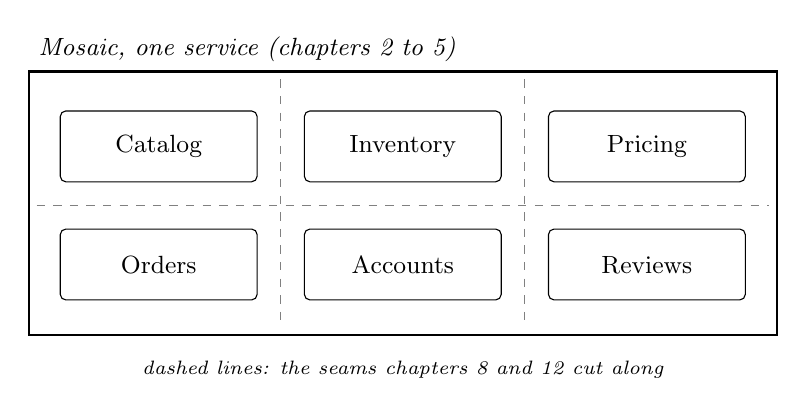
\begin{tikzpicture}[
    font=\small,
    dom/.style={draw, rounded corners=2pt, minimum width=25mm,
                minimum height=9mm, align=center},
    seam/.style={dashed, gray},
    note/.style={font=\scriptsize\itshape, align=center}
  ]

  \node[dom] (cat) at (0,0)      {Catalog};
  \node[dom] (inv) at (3.1,0)    {Inventory};
  \node[dom] (pri) at (6.2,0)    {Pricing};
  \node[dom] (ord) at (0,-1.5)   {Orders};
  \node[dom] (acc) at (3.1,-1.5) {Accounts};
  \node[dom] (rev) at (6.2,-1.5) {Reviews};

  % The one deployable everything starts inside.
  \draw[thick] (-1.65,0.95) rectangle (7.85,-2.4);
  \node[anchor=south west, font=\small\itshape] at (-1.65,0.95)
    {Mosaic, one service (chapters 2 to 5)};

  % Seams: where chapters 8 and 12 cut.
  \draw[seam] (1.55,0.85) -- (1.55,-2.3);
  \draw[seam] (4.65,0.85) -- (4.65,-2.3);
  \draw[seam] (-1.55,-0.75) -- (7.75,-0.75);

  \node[note, anchor=north] at (3.1,-2.6)
    {dashed lines: the seams chapters 8 and 12 cut along};

\end{tikzpicture}

  \caption{Mosaic starts as one service holding six domains. The dashed lines
  mark the seams the book eventually cuts along, and they are drawn where the
  data has natural owners rather than where the code happens to be
  convenient.}
  \label{fig:ch01-mosaic-domains}
\end{figure}

Chapters~\ref{ch:hotchocolate-quickly} through
\ref{ch:schema-design-that-survives-change} build Mosaic as a single
HotChocolate service on .NET, and build it properly. That word matters. A
federated graph assembled from services that were sloppy on their own is
worse than the monolith it replaced, because you have added a network between
the sloppy parts. Part I is about earning the right to distribute: resolvers
that batch, a schema that can absorb change, pagination that behaves. If you
already write GraphQL services for a living, that part will move quickly.

Here is where the pressure shows up. In the single-service version, Mosaic's
\code{Product} looks roughly like this:

\begin{graphqlsdl}
# Sketch, not code from the companion repo. Product as chapter 5
# leaves it, with all six domains' fields on one type.
type Product {
  id: ID!
  sku: String!
  title: String!
  description: String
  price: Money!
  availableQuantity: Int!
  averageRating: Float
  reviews(first: Int, after: String): ReviewConnection!
}
\end{graphqlsdl}

Nothing here is wrong. As a client-facing contract it is close to ideal: one
type, one query, everything a product page needs. The problem is that eight
fields are the responsibility of four different groups of people, and the
\code{Product} type is now a file all four of them edit. Add a currency to
\code{price} and you have touched the type that the reviews team is also
changing this sprint. That is the coordination cost from
section~\ref{sec:ch01-org-chart} arriving in a specific place, on a specific
line, and it will not be argued away with better process.

Chapter~\ref{ch:the-first-cut-extracting-catalog} takes the first slice,
moving Catalog out into its own subgraph while everything else stays put.
Chapter~\ref{ch:strangling-the-monolith} carves off the rest one domain at a
time, with the old monolith still serving traffic throughout, because that is
how this actually happens outside of books. By Part~VI, Mosaic is running as
a set of independently deployed services behind a router, with tracing that
crosses service boundaries and a CI pipeline that refuses to publish a
subgraph whose schema would break somebody else's query.

Mosaic runs on .NET~10 with HotChocolate~16 throughout, and lives in a
companion repository tagged per chapter, so you can check out the state of the
system at any point in the book rather than reconstructing it.
Appendix~\ref{app:toolchain} covers the setup and gives you a tour of the
repo. The code in this book comes
from that repository and compiles; where you see a fragment labelled as a
sketch, as in the listing above, it is there to make an argument and is not
something you should expect to find in a source file.
\index{Mosaic|)}

\section{Do you need this yet?}
\label{sec:ch01-do-you-need-this}

I have spent five sections describing a disease and naming companies that
caught it. Here is the part that gets left out of conference talks: plenty of
organisations operating at genuinely large scale looked at federation, and
decided against it, and were right.

\index{federation!when not to adopt}%
The most instructive example is Twitter's Core API Platform team, writing in
2021 about a schema that, by their own description, defined \enquote{the
entirety of our api data model} with roughly a thousand object types, a hundred
input types, and three hundred mutation fields, growing daily as \enquote{several
hundred developers across the company add fields and types}. That graph served
around 500,000 requests per second, and one of their most frequent queries was
2,500 lines long and returned 50,000 fields. When someone asked them directly
why they had not federated, the answer was that they did not need to:
\enquote{our underlying data layer (known as strato) is itself federated}, which
gave them \enquote{most of the perks of federation while also allowing us to
have a unified schema with strong network effects and without too many
performance gotchas}~\autocite{twitter2021unified}.

Read that last clause again, because it is a platform engineer at half a million
requests per second saying that a federated graph has performance
characteristics his unified schema does not have to deal with. It is also a
reminder that federation of the graph is not the only place you can put a seam.
They put theirs one layer down, in the data access tier, which is one of the
alternatives chapter~\ref{ch:do-you-actually-need-federation} takes seriously.

Zalando made a similar call for similar reasons. They run a unified graph across
their domains, but as a single service rather than a composed one, and Aditya
Pratap Singh was explicit that this is a trade rather than an oversight: they
\enquote{gain by keeping a single Graph in terms of tooling, deployment and
governance}~\autocite{singh2021zalando}. Tooling, deployment, and governance are
exactly the three things federation makes harder, and they are not glamorous
enough to make it into most architecture decisions.

\index{GitHub!GraphQL API}%
Then there is GitHub, which is the example I reach for when someone argues that
a schema can simply become too large for one service. I counted the published
GitHub GraphQL schema while writing this chapter: 1,807 named types and 6,809
fields on object and interface types, with 32 root query fields and 274
mutations~\autocite{github2026schema}. It is not versioned. It carries 1,258
deprecations, most of them with a removal date attached, governed by a published
policy that promises at least three months' notice and lands breaking changes on
quarter boundaries~\autocite{github2026breaking}. That is one schema, an order
of magnitude larger than most schemas anybody reading this owns, kept coherent
by a deprecation process rather than a distributed architecture. GraphQL's own
documentation notes that Meta, where the language was invented, has run a
monolithic GraphQL API since 2012~\autocite{graphqlorg2026federation}.

Schema size, then, is not the trigger. Neither is request volume. The trigger is
the number of teams that need to change the same part of the schema in the same
week, which is why the exercise at the end of this chapter asks you to count
that rather than to count fields.

\subsection*{What it costs}

If you do federate, here is the bill. I would rather you see it now than
discover it in Part~VI.

The router and the schema registry become production dependencies with their own
failure modes. Booking.com published the most useful account of this I know:
running close to a thousand gateway instances that fetched their schema roughly
8.3 million times a day, they hit a 24-hour window in which the failure rate for
schema delivery reached about 2.4 per cent against an expected 0.05 per cent,
and a gateway that cannot fetch a schema cannot roll
out~\autocite{ernst2022booking}. None of that is a criticism of federation. It
is what happens when composition becomes something your deploys depend on, and
it is work you were not doing before.

The performance surface is larger and harder to see into. At Netflix, where two
subgraph services between them handle over a million GraphQL queries per second,
Stephen Chambers described fixing a defect in the federation query-planning
layer, and the fix cut requests per second by 20 per cent and saved hundreds of
thousands of dollars~\autocite{chambers2026netflix}. That is a cost which had
been running silently until somebody went looking for it, in a layer that did
not exist before they federated.

The expertise cost is distributed rather than eliminated, which is easy to
misread as a saving. Netflix noted that in the monolith era only the Studio API
team needed to know GraphQL deeply, whereas afterwards \enquote{every DGS team
needs to build expertise in GraphQL}~\autocite{shikhare2020netflix2}. Airbnb,
who built a different answer to the same problem, put the structural version of
this well: \enquote{Federation distributes development by distributing
servers}~\autocite{tanner2026viaduct}. Hundreds of contributing teams means
hundreds of services to run, monitor, and page someone about.

\index{federation!maturity}%
It is worth noting who else says this. Netflix, the reference customer for the
entire idea, closed their own account of it by warning that federation
\enquote{is early in its maturity lifecycle and may not be the best fit for
every team or organization}, and that learning it, running a federation layer,
and carrying out the migration together \enquote{requires high commitment from
partner teams and seamless cross-functional
collaboration}~\autocite{shikhare2020netflix2}. GraphQL's own documentation is
blunter, saying federation \enquote{requires substantial infrastructure support,
including a dedicated team to manage the gateway, schema registry} and that
therefore \enquote{it's crucial to consider whether your organization truly
needs this level of complexity}~\autocite{graphqlorg2026federation}. When the
language's own home page tells you to think harder, that is not marketing.

\subsection*{A first pass}

So, a rough test, pending the real one in
chapter~\ref{ch:do-you-actually-need-federation}. Federation starts to earn its
cost when several teams own genuinely different domains inside one schema, when
those teams collide on the same types often enough that you can remember
specific incidents, when they need to deploy on their own schedules, and when
you already have the operational maturity to run another tier in production
without flinching. If instead you have one team, or several teams that rarely
touch each other's types, or nobody on call for a gateway, then the honest
answer is that your problems have cheaper solutions: a style guide, a
\code{CODEOWNERS} file, a deprecation policy like GitHub's, a modular monolith
with real internal boundaries.

Martin Fowler's advice to build the monolith first and split it once you can see
where the seams belong was published in 2015 and has aged
well~\autocite{fowler2015monolithfirst}. It is not unanimous, and the dissent is
worth reading: Stefan Tilkov argues on the same site that systems intended from
the start to be distributed are hard to retrofit into that shape
later~\autocite{tilkov2015dontstart}. For graphs specifically I still lean
Fowler's way, because a schema is unusually easy to carve later. The entity keys
that federation needs are mostly the identifiers you already have, and
chapter~\ref{ch:strangling-the-monolith} does exactly this carving without
downtime.

One last observation, offered as a caution rather than a conclusion. While
researching this chapter I looked for companies that had adopted federation and
then removed it, and found essentially none. That silence is real, but its cause
is not knowable from the outside. It might mean federation works. It might mean
that once a graph is composed, unpicking it costs more than living with it,
which is an argument for deciding carefully rather than a reassurance. Either
reading points the same direction: this is a decision worth making deliberately,
in advance, with your own numbers.

\section*{Your turn}

Every chapter from here ends with something to do, and from
chapter~\ref{ch:hotchocolate-quickly} onward that means checking out a tag from
the companion repository and running it. This one needs no code, because the
question this chapter raises is about your organisation rather than your
toolchain.

Pick a graph. If your team runs a GraphQL API, use that one, however small. If
you do not have one to hand, use GitHub's, which publishes its whole schema as a
single downloadable file~\autocite{github2026schema} alongside the
breaking-change policy that keeps it
manageable~\autocite{github2026breaking}. It is large, genuinely load bearing,
and deliberately not federated, which makes it a useful control case for
everything argued above. Answer the questions you can from the schema and the
policy; where you cannot, note what a maintainer would have to tell you.

\begin{enumerate}
  \item \textbf{Map the owners.} List the fields on \code{Query}. Next to each
  one, write the name of the team that would review a change to it. Count the
  fields where you cannot name a team, or where you can name three.

  \item \textbf{Measure the blast radius.} Take the type that appears in the
  most operations. How many separate features read it? If you added a required
  argument to one of its fields tomorrow, who finds out, and how?

  \item \textbf{Time a change.} Find the last field added to the schema. From
  the first commit to serving production traffic, how long did it take, and how
  many people had to agree? Separate the time spent building from the time
  spent waiting.

  \item \textbf{Test the coupling.} Can one domain in that schema ship a change
  to production without the others shipping too? If the answer is no, is that
  because of the schema, the deployment, or the database?

  \item \textbf{Count the queues.} Over the last quarter, how often did two
  teams need to change the same type in the same week?
\end{enumerate}

If your answers are dull, that is the most useful outcome available to you
here. Fields with one obvious owner, a change that ships in a day, one
deployable that everybody is happy to release: you have a healthy single graph
and no federation problem. Part~I of this book will still be worth your time,
and you can treat the rest as a map of where the road goes.

Keep the notes either way. Chapter~\ref{ch:do-you-actually-need-federation}
turns this audit into an actual decision, and by then you will have seen what
the alternative costs.

